\documentclass[1p]{elsarticle_modified}
%\bibliographystyle{elsarticle-num}

%\usepackage[colorlinks]{hyperref}
%\usepackage{abbrmath_seonhwa} %\Abb, \Ascr, \Acal ,\Abf, \Afrak
\usepackage{amsfonts}
\usepackage{amssymb}
\usepackage{amsmath}
\usepackage{amsthm}
\usepackage{scalefnt}
\usepackage{amsbsy}
\usepackage{kotex}
\usepackage{caption}
\usepackage{subfig}
\usepackage{color}
\usepackage{graphicx}
\usepackage{xcolor} %% white, black, red, green, blue, cyan, magenta, yellow
\usepackage{float}
\usepackage{setspace}
\usepackage{hyperref}

\usepackage{tikz}
\usetikzlibrary{arrows}

\usepackage{multirow}
\usepackage{array} % fixed length table
\usepackage{hhline}

%%%%%%%%%%%%%%%%%%%%%
\makeatletter
\renewcommand*\env@matrix[1][\arraystretch]{%
	\edef\arraystretch{#1}%
	\hskip -\arraycolsep
	\let\@ifnextchar\new@ifnextchar
	\array{*\c@MaxMatrixCols c}}
\makeatother %https://tex.stackexchange.com/questions/14071/how-can-i-increase-the-line-spacing-in-a-matrix
%%%%%%%%%%%%%%%

\usepackage[normalem]{ulem}

\newcommand{\msout}[1]{\ifmmode\text{\sout{\ensuremath{#1}}}\else\sout{#1}\fi}
%SOURCE: \msout is \stkout macro in https://tex.stackexchange.com/questions/20609/strikeout-in-math-mode

\newcommand{\cancel}[1]{
	\ifmmode
	{\color{red}\msout{#1}}
	\else
	{\color{red}\sout{#1}}
	\fi
}

\newcommand{\add}[1]{
	{\color{blue}\uwave{#1}}
}

\newcommand{\replace}[2]{
	\ifmmode
	{\color{red}\msout{#1}}{\color{blue}\uwave{#2}}
	\else
	{\color{red}\sout{#1}}{\color{blue}\uwave{#2}}
	\fi
}

\newcommand{\Sol}{\mathcal{S}} %segment
\newcommand{\D}{D} %diagram
\newcommand{\A}{\mathcal{A}} %arc


%%%%%%%%%%%%%%%%%%%%%%%%%%%%%5 test

\def\sl{\operatorname{\textup{SL}}(2,\Cbb)}
\def\psl{\operatorname{\textup{PSL}}(2,\Cbb)}
\def\quan{\mkern 1mu \triangleright \mkern 1mu}

\theoremstyle{definition}
\newtheorem{thm}{Theorem}[section]
\newtheorem{prop}[thm]{Proposition}
\newtheorem{lem}[thm]{Lemma}
\newtheorem{ques}[thm]{Question}
\newtheorem{cor}[thm]{Corollary}
\newtheorem{defn}[thm]{Definition}
\newtheorem{exam}[thm]{Example}
\newtheorem{rmk}[thm]{Remark}
\newtheorem{alg}[thm]{Algorithm}

\newcommand{\I}{\sqrt{-1}}
\begin{document}

%\begin{frontmatter}
%
%\title{Boundary parabolic representations of knots up to 8 crossings}
%
%%% Group authors per affiliation:
%\author{Yunhi Cho} 
%\address{Department of Mathematics, University of Seoul, Seoul, Korea}
%\ead{yhcho@uos.ac.kr}
%
%
%\author{Seonhwa Kim} %\fnref{s_kim}}
%\address{Center for Geometry and Physics, Institute for Basic Science, Pohang, 37673, Korea}
%\ead{ryeona17@ibs.re.kr}
%
%\author{Hyuk Kim}
%\address{Department of Mathematical Sciences, Seoul National University, Seoul 08826, Korea}
%\ead{hyukkim@snu.ac.kr}
%
%\author{Seokbeom Yoon}
%\address{Department of Mathematical Sciences, Seoul National University, Seoul, 08826,  Korea}
%\ead{sbyoon15@snu.ac.kr}
%
%\begin{abstract}
%We find all boundary parabolic representation of knots up to 8 crossings.
%
%\end{abstract}
%\begin{keyword}
%    \MSC[2010] 57M25 
%\end{keyword}
%
%\end{frontmatter}

%\linenumbers
%\tableofcontents
%
\newcommand\colored[1]{\textcolor{white}{\rule[-0.35ex]{0.8em}{1.4ex}}\kern-0.8em\color{red} #1}%
%\newcommand\colored[1]{\textcolor{white}{ #1}\kern-2.17ex	\textcolor{white}{ #1}\kern-1.81ex	\textcolor{white}{ #1}\kern-2.15ex\color{red}#1	}

{\Large $\underline{12a_{0773}~(K12a_{0773})}$}

\setlength{\tabcolsep}{10pt}
\renewcommand{\arraystretch}{1.6}
\vspace{1cm}\begin{tabular}{m{100pt}>{\centering\arraybackslash}m{274pt}}
\multirow{5}{120pt}{
	\centering
	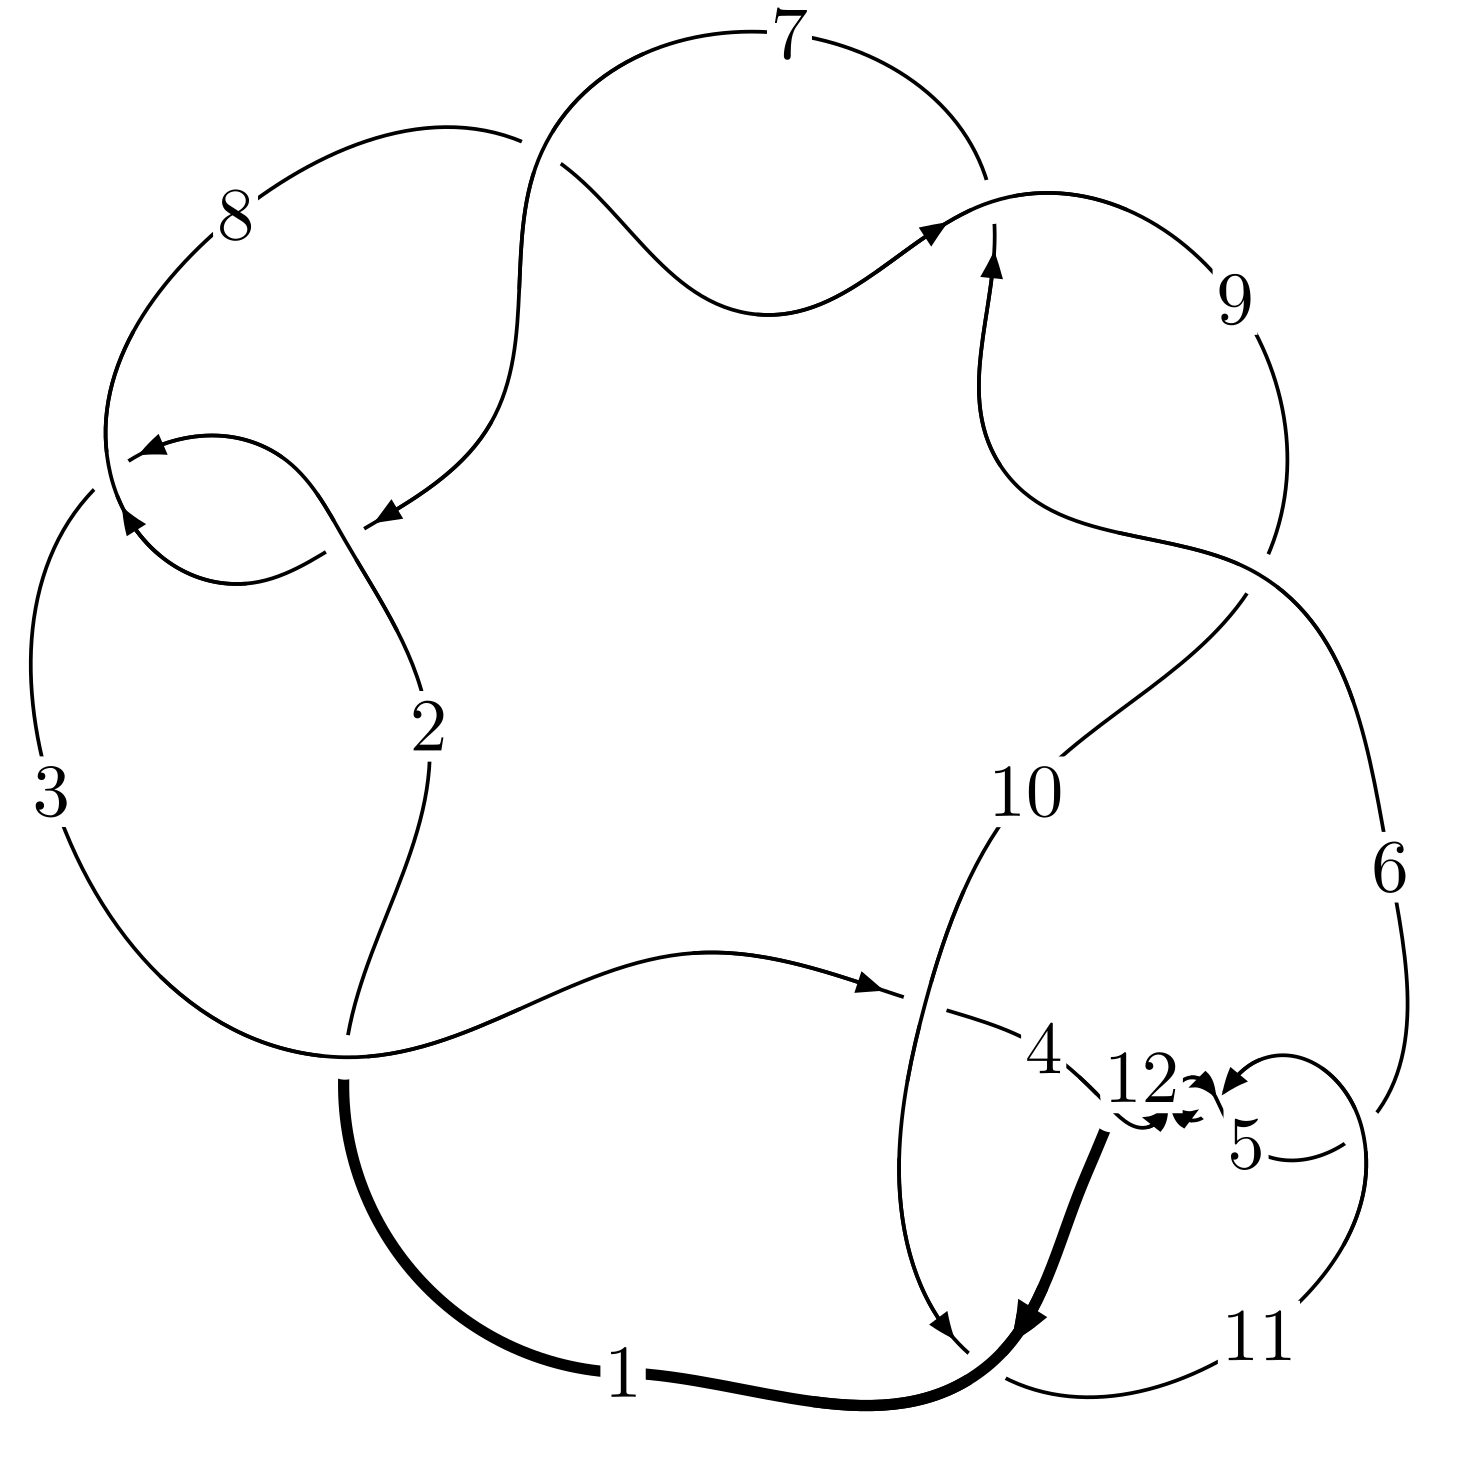
\includegraphics[width=112pt]{../../../GIT/diagram.site/Diagrams/png/1574_12a_0773.png}\\
\ \ \ A knot diagram\footnotemark}&
\allowdisplaybreaks
\textbf{Linearized knot diagam} \\
\cline{2-2}
 &
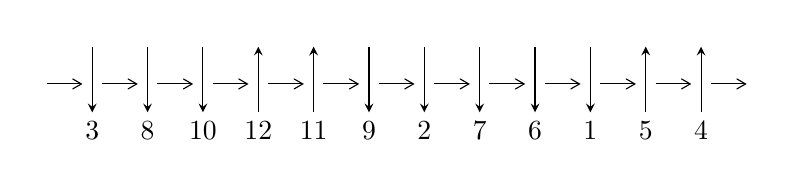
\begin{tikzpicture}[x=20pt, y=17pt]
	% nodes
	\node (C0) at (0, 0) {};
	\node (C1) at (1, 0) {};
	\node (C1U) at (1, +1) {};
	\node (C1D) at (1, -1) {3};

	\node (C2) at (2, 0) {};
	\node (C2U) at (2, +1) {};
	\node (C2D) at (2, -1) {8};

	\node (C3) at (3, 0) {};
	\node (C3U) at (3, +1) {};
	\node (C3D) at (3, -1) {10};

	\node (C4) at (4, 0) {};
	\node (C4U) at (4, +1) {};
	\node (C4D) at (4, -1) {12};

	\node (C5) at (5, 0) {};
	\node (C5U) at (5, +1) {};
	\node (C5D) at (5, -1) {11};

	\node (C6) at (6, 0) {};
	\node (C6U) at (6, +1) {};
	\node (C6D) at (6, -1) {9};

	\node (C7) at (7, 0) {};
	\node (C7U) at (7, +1) {};
	\node (C7D) at (7, -1) {2};

	\node (C8) at (8, 0) {};
	\node (C8U) at (8, +1) {};
	\node (C8D) at (8, -1) {7};

	\node (C9) at (9, 0) {};
	\node (C9U) at (9, +1) {};
	\node (C9D) at (9, -1) {6};

	\node (C10) at (10, 0) {};
	\node (C10U) at (10, +1) {};
	\node (C10D) at (10, -1) {1};

	\node (C11) at (11, 0) {};
	\node (C11U) at (11, +1) {};
	\node (C11D) at (11, -1) {5};

	\node (C12) at (12, 0) {};
	\node (C12U) at (12, +1) {};
	\node (C12D) at (12, -1) {4};
	\node (C13) at (13, 0) {};

	% arrows
	\draw[->,>={angle 60}]
	(C0) edge (C1) (C1) edge (C2) (C2) edge (C3) (C3) edge (C4) (C4) edge (C5) (C5) edge (C6) (C6) edge (C7) (C7) edge (C8) (C8) edge (C9) (C9) edge (C10) (C10) edge (C11) (C11) edge (C12) (C12) edge (C13) ;	\draw[->,>=stealth]
	(C1U) edge (C1D) (C2U) edge (C2D) (C3U) edge (C3D) (C4D) edge (C4U) (C5D) edge (C5U) (C6U) edge (C6D) (C7U) edge (C7D) (C8U) edge (C8D) (C9U) edge (C9D) (C10U) edge (C10D) (C11D) edge (C11U) (C12D) edge (C12U) ;
	\end{tikzpicture} \\
\hhline{~~} \\& 
\textbf{Solving Sequence} \\ \cline{2-2} 
 &
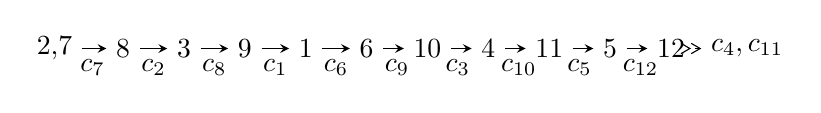
\begin{tikzpicture}[x=22pt, y=7pt]
	% node
	\node (A0) at (-1/8, 0) {2,7};
	\node (A1) at (1, 0) {8};
	\node (A2) at (2, 0) {3};
	\node (A3) at (3, 0) {9};
	\node (A4) at (4, 0) {1};
	\node (A5) at (5, 0) {6};
	\node (A6) at (6, 0) {10};
	\node (A7) at (7, 0) {4};
	\node (A8) at (8, 0) {11};
	\node (A9) at (9, 0) {5};
	\node (A10) at (10, 0) {12};
	\node (C1) at (1/2, -1) {$c_{7}$};
	\node (C2) at (3/2, -1) {$c_{2}$};
	\node (C3) at (5/2, -1) {$c_{8}$};
	\node (C4) at (7/2, -1) {$c_{1}$};
	\node (C5) at (9/2, -1) {$c_{6}$};
	\node (C6) at (11/2, -1) {$c_{9}$};
	\node (C7) at (13/2, -1) {$c_{3}$};
	\node (C8) at (15/2, -1) {$c_{10}$};
	\node (C9) at (17/2, -1) {$c_{5}$};
	\node (C10) at (19/2, -1) {$c_{12}$};
	\node (A11) at (45/4, 0) {$c_{4},c_{11}$};

	% edge
	\draw[->,>=stealth]	
	(A0) edge (A1) (A1) edge (A2) (A2) edge (A3) (A3) edge (A4) (A4) edge (A5) (A5) edge (A6) (A6) edge (A7) (A7) edge (A8) (A8) edge (A9) (A9) edge (A10) ;
	\draw[->>,>={angle 60}]	
	(A10) edge (A11);
\end{tikzpicture} \\ 

\end{tabular} \\

\footnotetext{
The image of knot diagram is generated by the software ``\textbf{Draw programme}" developed by Andrew Bartholomew(\url{http://www.layer8.co.uk/maths/draw/index.htm\#Running-draw}), where we modified some parts for our purpose(\url{https://github.com/CATsTAILs/LinksPainter}).
}\phantom \\ \newline 
\centering \textbf{Ideals for irreducible components\footnotemark of $X_{\text{par}}$} 
 
\begin{align*}
I^u_{1}&=\langle 
u^{45}+u^{44}+\cdots+u+1\rangle \\
\\
\end{align*}
\raggedright * 1 irreducible components of $\dim_{\mathbb{C}}=0$, with total 45 representations.\\
\footnotetext{All coefficients of polynomials are rational numbers. But the coefficients are sometimes approximated in decimal forms when there is not enough margin.}
\newpage
\renewcommand{\arraystretch}{1}
\centering \section*{I. $I^u_{1}= \langle u^{45}+u^{44}+\cdots+u+1 \rangle$}
\flushleft \textbf{(i) Arc colorings}\\
\begin{tabular}{m{7pt} m{180pt} m{7pt} m{180pt} }
\flushright $a_{2}=$&$\begin{pmatrix}0\\u\end{pmatrix}$ \\
\flushright $a_{7}=$&$\begin{pmatrix}1\\0\end{pmatrix}$ \\
\flushright $a_{8}=$&$\begin{pmatrix}1\\u^2\end{pmatrix}$ \\
\flushright $a_{3}=$&$\begin{pmatrix}- u\\- u^3+u\end{pmatrix}$ \\
\flushright $a_{9}=$&$\begin{pmatrix}- u^2+1\\u^2\end{pmatrix}$ \\
\flushright $a_{1}=$&$\begin{pmatrix}u^3\\u^5- u^3+u\end{pmatrix}$ \\
\flushright $a_{6}=$&$\begin{pmatrix}u^4- u^2+1\\- u^4\end{pmatrix}$ \\
\flushright $a_{10}=$&$\begin{pmatrix}- u^6+u^4-2 u^2+1\\u^6+u^2\end{pmatrix}$ \\
\flushright $a_{4}=$&$\begin{pmatrix}u^{15}-2 u^{13}+6 u^{11}-8 u^9+10 u^7-8 u^5+4 u^3-2 u\\- u^{15}+u^{13}-4 u^{11}+3 u^9-4 u^7+2 u^5-2 u^3+u\end{pmatrix}$ \\
\flushright $a_{11}=$&$\begin{pmatrix}- u^{14}+u^{12}-4 u^{10}+3 u^8-4 u^6+2 u^4-2 u^2+1\\- u^{16}+2 u^{14}-6 u^{12}+8 u^{10}-10 u^8+8 u^6-4 u^4+2 u^2\end{pmatrix}$ \\
\flushright $a_{5}=$&$\begin{pmatrix}u^{34}-3 u^{32}+\cdots+u^2+1\\u^{36}-4 u^{34}+\cdots-18 u^6+3 u^4\end{pmatrix}$ \\
\flushright $a_{12}=$&$\begin{pmatrix}- u^{35}+4 u^{33}+\cdots+18 u^5-3 u^3\\u^{35}-3 u^{33}+\cdots+u^3+u\end{pmatrix}$\\&\end{tabular}
\flushleft \textbf{(ii) Obstruction class $= -1$}\\~\\
\flushleft \textbf{(iii) Cusp Shapes $= -4 u^{44}+20 u^{42}+\cdots-4 u-6$}\\~\\
\newpage\renewcommand{\arraystretch}{1}
\flushleft \textbf{(iv) u-Polynomials at the component}\newline \\
\begin{tabular}{m{50pt}|m{274pt}}
Crossings & \hspace{64pt}u-Polynomials at each crossing \\
\hline $$\begin{aligned}c_{1},c_{6},c_{8}\\c_{9}\end{aligned}$$&$\begin{aligned}
&u^{45}+9 u^{44}+\cdots- u+1
\end{aligned}$\\
\hline $$\begin{aligned}c_{2},c_{7}\end{aligned}$$&$\begin{aligned}
&u^{45}+u^{44}+\cdots+u+1
\end{aligned}$\\
\hline $$\begin{aligned}c_{3}\end{aligned}$$&$\begin{aligned}
&u^{45}+u^{44}+\cdots+21 u+1
\end{aligned}$\\
\hline $$\begin{aligned}c_{4},c_{5},c_{11}\\c_{12}\end{aligned}$$&$\begin{aligned}
&u^{45}+u^{44}+\cdots+3 u+1
\end{aligned}$\\
\hline $$\begin{aligned}c_{10}\end{aligned}$$&$\begin{aligned}
&u^{45}-11 u^{44}+\cdots-3 u-3
\end{aligned}$\\
\hline
\end{tabular}\\~\\
\newpage\renewcommand{\arraystretch}{1}
\flushleft \textbf{(v) Riley Polynomials at the component}\newline \\
\begin{tabular}{m{50pt}|m{274pt}}
Crossings & \hspace{64pt}Riley Polynomials at each crossing \\
\hline $$\begin{aligned}c_{1},c_{6},c_{8}\\c_{9}\end{aligned}$$&$\begin{aligned}
&y^{45}+55 y^{44}+\cdots+7 y-1
\end{aligned}$\\
\hline $$\begin{aligned}c_{2},c_{7}\end{aligned}$$&$\begin{aligned}
&y^{45}-9 y^{44}+\cdots- y-1
\end{aligned}$\\
\hline $$\begin{aligned}c_{3}\end{aligned}$$&$\begin{aligned}
&y^{45}- y^{44}+\cdots+191 y-1
\end{aligned}$\\
\hline $$\begin{aligned}c_{4},c_{5},c_{11}\\c_{12}\end{aligned}$$&$\begin{aligned}
&y^{45}+51 y^{44}+\cdots- y-1
\end{aligned}$\\
\hline $$\begin{aligned}c_{10}\end{aligned}$$&$\begin{aligned}
&y^{45}+3 y^{44}+\cdots+507 y-9
\end{aligned}$\\
\hline
\end{tabular}\\~\\
\newpage\flushleft \textbf{(vi) Complex Volumes and Cusp Shapes}
$$\begin{array}{c|c|c}  
\text{Solutions to }I^u_{1}& \I (\text{vol} + \sqrt{-1}CS) & \text{Cusp shape}\\
 \hline 
\begin{aligned}
u &= \phantom{-}0.842523 + 0.539612 I\end{aligned}
 & \phantom{-}1.63617 - 3.33410 I & -0.33334 + 4.44336 I \\ \hline\begin{aligned}
u &= \phantom{-}0.842523 - 0.539612 I\end{aligned}
 & \phantom{-}1.63617 + 3.33410 I & -0.33334 - 4.44336 I \\ \hline\begin{aligned}
u &= -0.745790 + 0.649514 I\end{aligned}
 & -3.25288 + 2.39871 I & -2.89131 - 3.55564 I \\ \hline\begin{aligned}
u &= -0.745790 - 0.649514 I\end{aligned}
 & -3.25288 - 2.39871 I & -2.89131 + 3.55564 I \\ \hline\begin{aligned}
u &= -0.893450 + 0.533806 I\end{aligned}
 & \phantom{-}0.35918 + 6.76103 I & -4.58151 - 10.24409 I \\ \hline\begin{aligned}
u &= -0.893450 - 0.533806 I\end{aligned}
 & \phantom{-}0.35918 - 6.76103 I & -4.58151 + 10.24409 I \\ \hline\begin{aligned}
u &= \phantom{-}0.882706 + 0.368441 I\end{aligned}
 & -9.18323 - 0.52895 I & -10.64212 + 3.60551 I \\ \hline\begin{aligned}
u &= \phantom{-}0.882706 - 0.368441 I\end{aligned}
 & -9.18323 + 0.52895 I & -10.64212 - 3.60551 I \\ \hline\begin{aligned}
u &= \phantom{-}0.924753 + 0.528045 I\end{aligned}
 & -7.25615 - 8.99421 I & -7.47706 + 8.23216 I \\ \hline\begin{aligned}
u &= \phantom{-}0.924753 - 0.528045 I\end{aligned}
 & -7.25615 + 8.99421 I & -7.47706 - 8.23216 I \\ \hline\begin{aligned}
u &= -0.915632 + 0.085731 I\end{aligned}
 & -10.66890 + 4.29803 I & -13.41929 - 4.05209 I \\ \hline\begin{aligned}
u &= -0.915632 - 0.085731 I\end{aligned}
 & -10.66890 - 4.29803 I & -13.41929 + 4.05209 I \\ \hline\begin{aligned}
u &= -0.798279 + 0.412042 I\end{aligned}
 & -1.42195 + 1.48989 I & -9.20204 - 3.10031 I \\ \hline\begin{aligned}
u &= -0.798279 - 0.412042 I\end{aligned}
 & -1.42195 - 1.48989 I & -9.20204 + 3.10031 I \\ \hline\begin{aligned}
u &= \phantom{-}0.622618 + 0.607896 I\end{aligned}
 & \phantom{-}2.34985 - 1.00131 I & \phantom{-}2.25214 + 3.75135 I \\ \hline\begin{aligned}
u &= \phantom{-}0.622618 - 0.607896 I\end{aligned}
 & \phantom{-}2.34985 + 1.00131 I & \phantom{-}2.25214 - 3.75135 I \\ \hline\begin{aligned}
u &= \phantom{-}0.860336 + 0.082675 I\end{aligned}
 & -2.96104 - 2.56413 I & -12.15035 + 6.37098 I \\ \hline\begin{aligned}
u &= \phantom{-}0.860336 - 0.082675 I\end{aligned}
 & -2.96104 + 2.56413 I & -12.15035 - 6.37098 I \\ \hline\begin{aligned}
u &= \phantom{-}0.500299 + 0.676887 I\end{aligned}
 & -5.89698 + 4.51199 I & -3.83830 - 2.27659 I \\ \hline\begin{aligned}
u &= \phantom{-}0.500299 - 0.676887 I\end{aligned}
 & -5.89698 - 4.51199 I & -3.83830 + 2.27659 I \\ \hline\begin{aligned}
u &= -0.545239 + 0.640437 I\end{aligned}
 & \phantom{-}1.47015 - 2.35216 I & -0.76426 + 3.93836 I \\ \hline\begin{aligned}
u &= -0.545239 - 0.640437 I\end{aligned}
 & \phantom{-}1.47015 + 2.35216 I & -0.76426 - 3.93836 I \\ \hline\begin{aligned}
u &= -0.753905\phantom{ +0.000000I}\end{aligned}
 & -1.22216\phantom{ +0.000000I} & -7.16390\phantom{ +0.000000I} \\ \hline\begin{aligned}
u &= -0.913783 + 0.849175 I\end{aligned}
 & -2.09514 + 3.15874 I & -6.19428 - 2.57138 I \\ \hline\begin{aligned}
u &= -0.913783 - 0.849175 I\end{aligned}
 & -2.09514 - 3.15874 I & -6.19428 + 2.57138 I \\ \hline\begin{aligned}
u &= \phantom{-}0.923803 + 0.877811 I\end{aligned}
 & \phantom{-}6.39657 - 3.24843 I & -4.00000 + 2.33788 I \\ \hline\begin{aligned}
u &= \phantom{-}0.923803 - 0.877811 I\end{aligned}
 & \phantom{-}6.39657 + 3.24843 I & -4.00000 - 2.33788 I \\ \hline\begin{aligned}
u &= -0.888807 + 0.915163 I\end{aligned}
 & \phantom{-}2.17300 - 5.40200 I & -4.00000 + 2.07857 I \\ \hline\begin{aligned}
u &= -0.888807 - 0.915163 I\end{aligned}
 & \phantom{-}2.17300 + 5.40200 I & -4.00000 - 2.07857 I \\ \hline\begin{aligned}
u &= \phantom{-}0.897839 + 0.910766 I\end{aligned}
 & \phantom{-}9.68761 + 2.81350 I & \phantom{-0.000000 } 0. - 3.36569 I\\
 \hline 
 \end{array}$$\newpage$$\begin{array}{c|c|c}  
\text{Solutions to }I^u_{1}& \I (\text{vol} + \sqrt{-1}CS) & \text{Cusp shape}\\
 \hline 
\begin{aligned}
u &= \phantom{-}0.897839 - 0.910766 I\end{aligned}
 & \phantom{-}9.68761 - 2.81350 I & \phantom{-0.000000 -}0. + 3.36569 I \\ \hline\begin{aligned}
u &= -0.908434 + 0.905373 I\end{aligned}
 & \phantom{-}10.78900 + 1.09718 I & \phantom{-0.000000 } 0. - 2.47582 I \\ \hline\begin{aligned}
u &= -0.908434 - 0.905373 I\end{aligned}
 & \phantom{-}10.78900 - 1.09718 I & \phantom{-0.000000 -}0. + 2.47582 I \\ \hline\begin{aligned}
u &= \phantom{-}0.932398 + 0.899940 I\end{aligned}
 & \phantom{-}5.98919 - 3.31737 I & -4.00000 + 2.40847 I \\ \hline\begin{aligned}
u &= \phantom{-}0.932398 - 0.899940 I\end{aligned}
 & \phantom{-}5.98919 + 3.31737 I & -4.00000 - 2.40847 I \\ \hline\begin{aligned}
u &= -0.951494 + 0.884176 I\end{aligned}
 & \phantom{-}10.64970 + 5.50488 I & \phantom{-0.000000 } 0 \\ \hline\begin{aligned}
u &= -0.951494 - 0.884176 I\end{aligned}
 & \phantom{-}10.64970 - 5.50488 I & \phantom{-0.000000 } 0 \\ \hline\begin{aligned}
u &= \phantom{-}0.961169 + 0.879776 I\end{aligned}
 & \phantom{-}9.48304 - 9.41748 I & \phantom{-0.000000 -}0. + 8.04677 I \\ \hline\begin{aligned}
u &= \phantom{-}0.961169 - 0.879776 I\end{aligned}
 & \phantom{-}9.48304 + 9.41748 I & \phantom{-0.000000 } 0. - 8.04677 I \\ \hline\begin{aligned}
u &= -0.968830 + 0.875878 I\end{aligned}
 & \phantom{-}1.91452 + 12.00600 I & \phantom{-0.000000 } 0. - 6.72542 I \\ \hline\begin{aligned}
u &= -0.968830 - 0.875878 I\end{aligned}
 & \phantom{-}1.91452 - 12.00600 I & \phantom{-0.000000 -}0. + 6.72542 I \\ \hline\begin{aligned}
u &= \phantom{-}0.192606 + 0.558254 I\end{aligned}
 & -7.18221 - 2.67775 I & -4.03487 + 2.63740 I \\ \hline\begin{aligned}
u &= \phantom{-}0.192606 - 0.558254 I\end{aligned}
 & -7.18221 + 2.67775 I & -4.03487 - 2.63740 I \\ \hline\begin{aligned}
u &= -0.134361 + 0.422733 I\end{aligned}
 & -0.031442 + 1.214490 I & -0.60670 - 5.55927 I \\ \hline\begin{aligned}
u &= -0.134361 - 0.422733 I\end{aligned}
 & -0.031442 - 1.214490 I & -0.60670 + 5.55927 I\\
 \hline 
 \end{array}$$\newpage
\newpage\renewcommand{\arraystretch}{1}
\centering \section*{ II. u-Polynomials}
\begin{tabular}{m{50pt}|m{274pt}}
Crossings & \hspace{64pt}u-Polynomials at each crossing \\
\hline $$\begin{aligned}c_{1},c_{6},c_{8}\\c_{9}\end{aligned}$$&$\begin{aligned}
&u^{45}+9 u^{44}+\cdots- u+1
\end{aligned}$\\
\hline $$\begin{aligned}c_{2},c_{7}\end{aligned}$$&$\begin{aligned}
&u^{45}+u^{44}+\cdots+u+1
\end{aligned}$\\
\hline $$\begin{aligned}c_{3}\end{aligned}$$&$\begin{aligned}
&u^{45}+u^{44}+\cdots+21 u+1
\end{aligned}$\\
\hline $$\begin{aligned}c_{4},c_{5},c_{11}\\c_{12}\end{aligned}$$&$\begin{aligned}
&u^{45}+u^{44}+\cdots+3 u+1
\end{aligned}$\\
\hline $$\begin{aligned}c_{10}\end{aligned}$$&$\begin{aligned}
&u^{45}-11 u^{44}+\cdots-3 u-3
\end{aligned}$\\
\hline
\end{tabular}\newpage\renewcommand{\arraystretch}{1}
\centering \section*{ III. Riley Polynomials}
\begin{tabular}{m{50pt}|m{274pt}}
Crossings & \hspace{64pt}Riley Polynomials at each crossing \\
\hline $$\begin{aligned}c_{1},c_{6},c_{8}\\c_{9}\end{aligned}$$&$\begin{aligned}
&y^{45}+55 y^{44}+\cdots+7 y-1
\end{aligned}$\\
\hline $$\begin{aligned}c_{2},c_{7}\end{aligned}$$&$\begin{aligned}
&y^{45}-9 y^{44}+\cdots- y-1
\end{aligned}$\\
\hline $$\begin{aligned}c_{3}\end{aligned}$$&$\begin{aligned}
&y^{45}- y^{44}+\cdots+191 y-1
\end{aligned}$\\
\hline $$\begin{aligned}c_{4},c_{5},c_{11}\\c_{12}\end{aligned}$$&$\begin{aligned}
&y^{45}+51 y^{44}+\cdots- y-1
\end{aligned}$\\
\hline $$\begin{aligned}c_{10}\end{aligned}$$&$\begin{aligned}
&y^{45}+3 y^{44}+\cdots+507 y-9
\end{aligned}$\\
\hline
\end{tabular}
\vskip 2pc
\end{document}